%--------------------------------------------------------------------
% Эта преамбула с комментариями для написания лабораторных работ по
% физике. В еe основе информация из книги С. М. Львовского "Набор и
% верстка в пакете Latex", а также материалы по курсу "Документы и
% презентации в Latex" от ВШЭ https://www.coursera.org/learn/latex. Ну
% и мой опыт (1 год и 16 лабораторных работ + 2 Вопроса по выбору)
% Автор - Баринов Леонид
% Дата - 06.08.2019
%--------------------------------------------------------------------
%--------------------------------------------------------------------
% Для начала необходимо определиться с типом документа. Оптимальный
% (на мой взгляд) вариант - article. Также существуют типы book,
% report, proc и другие. Также в необязательном аргументе можно
% указать тип страницы и размер шрифта. Стандарт по умолчанию - А4 и
% 12 (иногда 10) шрифт. Необязательный аргумент шрифта может принимать
% только 3 параметра - 10, 11, 12 (pt).

\documentclass[a4paper, 12pt]{article}

%--------------------------------------------------------------------
% Чтобы использовать другие размеры шрифта используется пакет
% extsizes. Он позволяет указывать в \documentclass такие размеры - 8,
% 9, 10, 11, 12, 14, 17, 20 (pt). При указании других размеров могут
% возникать различные проблемы.

\usepackage{extsizes}

%--------------------------------------------------------------------
% Необходимо определиться с кодировкой документа. Идеального варианта
% для русского языка не существует - каждый чем-то немного плох. Для
% особо интересующихся - Приложение И в 5 издании книги Львовского. Я
% воспользовался вариантом, предлагаемым на курсе по Latex от ВШЭ.

\usepackage[T2A]{fontenc}
\usepackage[utf8]{inputenc}

%--------------------------------------------------------------------
% Для соблюдения типографских традиций (оказывается такие существуют)
% различных стран создан пакет babel. Самое заметное его действие -
% latex научиться переносить слова того языка, который вы укажите.
% Можно указать несколько языков через запятую. Основной язык
% документа указывается последним.

\usepackage[english,russian]{babel}

%--------------------------------------------------------------------
% Перейдем к заданию полей документа. Есть несколько способов, но
% самый простой из них - это воспользоваться пакетом geometry, который
% позволяет определить все поля документа (начиная с краев листа, что
% важно, так как некоторые другие способы позволяют это сделать только
% косвенно)

\usepackage{geometry}
\geometry{top=25mm}
\geometry{bottom=35mm}
\geometry{left=35mm}
\geometry{right=20mm}

%--------------------------------------------------------------------
% От полей логично перейти к колонтитулам. Тут нам поможет пакет
% fancyhdr. Для него существует 6 колонтитулов - верхний, левый;
% верхний, по центру; верхний, правый и такие же нижние. По умолчанию
% номер страницы находится снизу по центру, а также существует
% линейка, очерчивающие верхний колонтитул. Мне показалось интересным
% сделать колонтитулы схожие с колонтитулами в лабнике. 

\usepackage{fancyhdr}
\pagestyle{fancy}
\renewcommand{\sectionmark}[1]{\markboth{#1}{}} 
% \renewcommand{\headrulewidth}{0mm} % Если необходимо убрать линейку,
% или изменить ее длину
% \lfoot{} % Нижний левый
% \rfoot{} % Нижний правый
% \rhead{} % Верхний правый
% \chead{} % Верхний в центре
\lhead{\thepage} % Номер страницы в левом верхнем углу
\cfoot{} % Оставить нижний колонтитул без цифры

%--------------------------------------------------------------------
% Самое время научиться работать с формулами. А точнее добавить пакеты
% от Американского математического общества, которые позволять
% пользоваться большим количеством математических символов.

\usepackage{amsmath,amsfonts,amssymb,amsthm,mathtools}

%--------------------------------------------------------------------
% Также очень хочется пользоваться русскими буквами в формулах, для
% этого подключаем пакет mathtext, который добавляет окружение
% \text{}. Внутри него можно писать русские буквы в математическом
% режиме.

\usepackage{mathtext}

%--------------------------------------------------------------------
% Большим преимуществом вашего pdf документа будет возможность поиска
% в нем по словам или буквами. (Например, в Ивановнике это
% невозможно)

\usepackage{cmap}

%--------------------------------------------------------------------
% Куда же в физике без картинок и графиков? Давайте исправим
% эту недоработку

\usepackage{graphicx}
\graphicspath{images/} % Необходимо, если рисунки
% находятся в другой папке

%--------------------------------------------------------------------
% graphicx не позволяет вставлять обтекаемые рисунки, но на
% практике они очень нужны. Для этого существует пакет wrapfig

\usepackage{wrapfig}

%--------------------------------------------------------------------
% latex вставляет рисунки по определенному алгоритму. Его,
% конечно, можно менять, но это не настолько просто. Как
% правило, хочется, чтобы картинка располагалась там, где мы это
% указали в коде. Для этого существует несколько пакетов, один из
% них floatrow. Он позволяет для окружения figure указывать
% необязательный аргумент - H (именно большое h), что на latex'овском
% языке означает: вставить картинку здесь и только здесь. (даже если
% облик документа несколько пострадает)

\usepackage{floatrow}

%--------------------------------------------------------------------
% По правилам оформления рисунок всегда должен быть подписан. Для
% этого существует команда \caption{}. Но обычные настройки caption
% меня не совсем устроили. Хотелось сделать подпись меньше
% основного шрифта, а также слово Рис жирным и использовать
% разделитель точку, а не двоеточие. В этом помогает пакет,
% который называется caption (совпадение?)

\usepackage[margin=10pt,font=small,labelfont=bf,labelsep=period]{caption}

%--------------------------------------------------------------------
% Последним важным пунктом остались таблицы. Ведь куда-то нужно
% заносить результаты измерений. На данный момент во время выполнения
% лабораторных работ я заношу результаты в таблицу excel, а потом с
% помощью сайта www.tablesgenerator.com превращаю в таблицу latex и
% дооформляю.

\usepackage{array,tabularx,tabulary,booktabs}

%--------------------------------------------------------------------
% После excel есть ощущения, что везде объединить колонки или строки
% легко. В latex не совсем так. Помогают пакеты multirow, multicol. 

\usepackage{multirow}
\usepackage{multicol}

%--------------------------------------------------------------------
% Иногда могут потребоваться длинные таблицы на несколько страниц.
% Обычные таблицы latex воспринимает как одну букву. И
% становиться понятно, почему возникают проблемы при переносе
% обычной таблицы. (Ведь нельзя же перенести одну букву!). Поэтому
% вместо обычной таблицы нужна длинная таблица.

\usepackage{longtable}

%--------------------------------------------------------------------
% Часто в таблице хочется сделать перенос текста или формулы. Просто
% так это сделать не получиться из-за синтаксиса tabular. Для этого
% каждый раз необходимо создавать новое окружение tabular, что
% утомительно. Поэтому можно ввести команду \specialcell
% (назвать можно по-любому)
    
\newcommand{\specialcell}[2][c]{%
	\begin{tabular}[#1]{@{}c{}}#2\end{tabular}}

%--------------------------------------------------------------------
% Когда в таблице много колонок и строк, кажется, что они находятся
% слишком близко к друг другу. Можно переопределить
% несколько параметров, чтобы выглядело лучше. Это можно сделать либо
% в преамбуле, либо непосредственно в документе. Первое
% переопределение отвечает за интервал между строками, второе за
% интервал между колонками

% \renewcommand{\arraystretch}{1.8} 
% \renewcommand{\tabcolsep}{1cm} 

%--------------------------------------------------------------------
% В русской типографской традиции принято начинать каждый новый абзац
% с красной строки. Даже первый после заголовка (или подзаголовка).
% Чтобы каждый раз не ставить красную строку вручную существует пакет
% indentfirst

\usepackage{indentfirst}

%--------------------------------------------------------------------
% Некоторые модификаторы начертания

\usepackage{soul}
\usepackage{soulutf8}
 
\begin{document}
\thispagestyle{empty}
\begin{center}
    \textit{Федеральное государственное автономное образовательное\\ учреждение высшего образования }

    \vspace{0.5ex}

        \textbf{«Московский физико-технический институт\\ (национальный исследовательский университет)»}
\end{center}

\vspace{10ex}

\begin{center}
    \vspace{13ex}

    \so{\textbf{Лабораторная работа №_._._}}

    \vspace{1ex}

    по курсу общей физики

    на тему:

    \textbf{\textit{<<>>}}

    \vspace{30ex}

    \begin{flushright}
        \noindent
        \textit{Работу выполнил:}\\  
        \textit{Баринов Леонид \\(группа Б02-827)}
    \end{flushright}
    \vfill
    Долгопрудный \\2019
\newpage
\setcounter{page}{1}
\fancyhead[R]{\nouppercase{\leftmark}}	
\end{center}

\section{Аннотация}
В работе будет исследована: зависимость
периода свободных колебаний контура от
ёмкости; зависимость логарифмического
декремента затухания от сопротивления.
Будет определено критическое
сопротивление и добротность контура.
\section{Оборудование}
\textbf{В работе используются:} генератор импульсов, электронное реле, магазин сопротивлений,
магазин емкостей, индуктивность, электронный осциллограф с разделительной панелью, измеритель
LCR.
\subsection*{Экспериментальная установка}
На Рис. 1 приведена схема для исследования свободных колебаний в контуре, содержащем постоянную
индуктивность $I$ и переменные ёмкость $C$ и сопротивление $R$. Колебания наблюдаются на экране
осциллографа.

Для периодического возбуждения колебаний в контуре используется генератор импульсов Г5-54. С выхода
генератора по коаксиальному кабелю импульсы поступают на колебательный контур через электронное
реле, смонтированное в отдельном блоке (или на выходе генератора). Реле содержит диодный тиристор
$D$ и ограничительный резистор $R_1$.
\begin{figure}[H]
    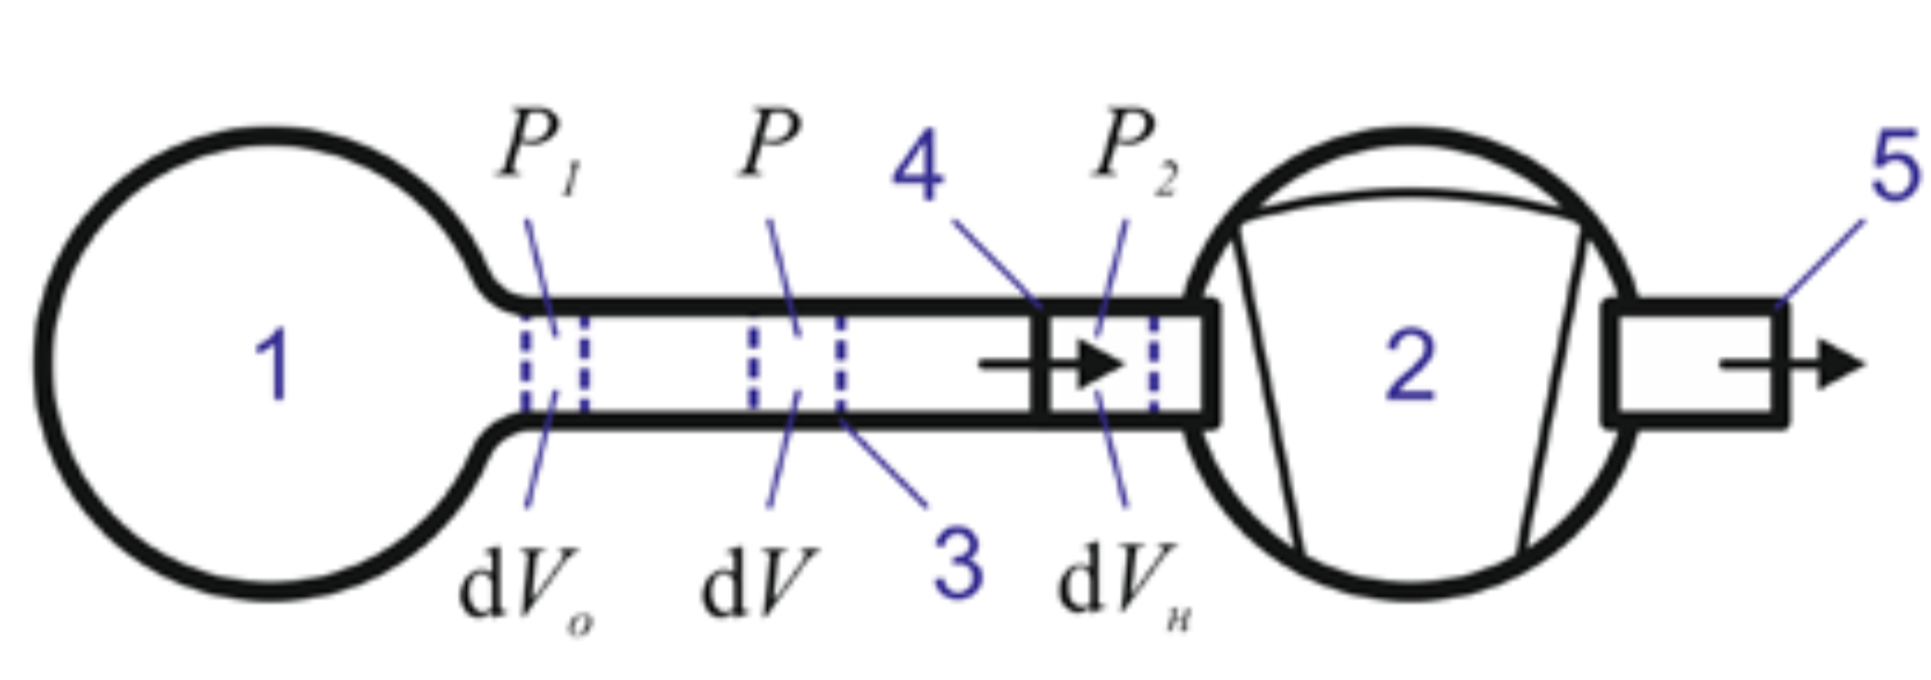
\includegraphics[width=\linewidth]{1}
    \captionsetup{justification =
    centering}
    \caption{Схема установки для
    исследования свободных колебаний}
\end{figure}
Импульсы заряжают конденсатор $C$. После
каждого импульса генератор отключается
от колебательного контура, и в контуре
возникают свободные затухающие
колебания. Входное сопротивление
осциллографа велико ($\sim 1\ \text{МОм}$), так что
его влиянием на контур можно пренебречь.
Для получения устойчивой картины
затухающих колебаний используется режим
ждущей развёртки с синхронизацией
внешними импульсами, поступающими с
выхода синхроимпульсы генератора. 

\section{Результаты измерений и обработка результатов}
Установим на магазине сопротивлений
величину $R$ = 0; на магазине емкостей~
-- величину $C = 0,02\ \text{мкФ}$.
Прокалибруем горизонтальную ось
осциллографа по известному периоду
повторения импульсов. Подберем частоту
развертки ЭO, при которой
расстояние $x_0$ между импульсами,
поступающими с генератора, занимает
почти весь экран
\[
    x_0 = 50\pm 2\ \text{дел}
\]

Проведем измерения расстояния $x$,
которое занимают несколько полных
периодов $n$. Зная $T_0 = 0,01\
\text{с}$ и $x_0$, рассчитаем период
колебаний по формуле $T~ =~ T_0x/(nx_0)$.
\renewcommand{\arraystretch}{1.1} 
\begin{table}[H]
\begin{tabular}{|c|c|c|c|c|}
\hline
$C, \ \text{мкФ}$    & $x, \ \text{дел}$
& $n$  & $T, \text{мс}$    & $\Delta T,
\ \text{мс}$   \\ \hline
0,10  & 50 & 13 & 0,77 & 0,03 \\ \hline
0,20  & 50 & 9  & 1,11 & 0,04 \\ \hline
0,25 & 29 & 5  & 1,16 & 0,08 \\ \hline
0,30  & 19 & 3  & 1,27 & 0,13 \\ \hline
0,40  & 15 & 2  & 1,50 & 0,20 \\ \hline
0,45 & 31 & 4  & 1,55 & 0,10 \\ \hline
0,50  & 17 & 2  & 1,70 & 0,20 \\ \hline
0,60  & 27 & 3  & 1,80 & 0,13 \\ \hline
0,65 & 28 & 3  & 1,87 & 0,13 \\ \hline
0,70  & 39 & 4  & 1,95 & 0,10 \\ \hline
0,80  & 32 & 3  & 2,13 & 0,13 \\ \hline
0,90  & 33 & 3  & 2,20 & 0,13 \\ \hline
\end{tabular}
\captionsetup{justification=centering}
\caption{Измерение периодов колебаний
$T$ при различных значениях емкостей
конденсатора $C$}
\end{table}

Найдем сопротивление магазина
$R_\text{кр}$, при котором колебательный
режим переходит в апериодический.
\[
    R_\text{кр} = 9800 \pm 800 \
    \text{Ом}
\]

Установим сопротивление $R \approx
0,1R_\text{кр}$. Получим на экране
картину затухающих колебаний. Рассчитаем
логарифмический декремент затухания
$\Theta$ по формуле:
\[
    \Theta =
    \frac{1}{n}\ln\frac{U_k}{U_{k+n}}
\]
где $n$ -- целое число периодов,
разделяющих измеренные значения амплитуд.

Проведем измерения для значений $R$ в
интервале $(0,1 - 0,3)R_\text{кр}$.

\begin{table}[H]
\begin{tabular}{|c|c|c|c|c|c|}
\hline
$U_k, \ \text{дел}$ &
\begin{tabular}{c}$U_{k+n},$ \\
$\text{дел}$\end{tabular} & $n$& $R, \
\text{Ом}$ &
$\Theta$ & $\Delta\Theta$    \\ \hline
22 & 1   & 5 & 960  & 0,62 & 0,06 \\ \hline
20 & 1   & 4 & 1152 & 0,75 & 0,07 \\ \hline
18 & 1   & 3 & 1440 & 0,96 & 0,11 \\ \hline
15 & 1,5 & 2 & 1728 & 1,15 & 0,15 \\ \hline
15 & 1   & 2 & 1920 & 1,35 & 0,18 \\ \hline
14 & 1   & 2 & 2112 & 1,32 & 0,19 \\ \hline
13 & 2,5 & 1 & 2400 & 1,65 & 0,25 \\ \hline
11 & 1,5 & 1 & 2880 & 1,99 & 0,36 \\ \hline
\end{tabular}
\captionsetup{justification=centering}
\caption{Амплитуды $U_k$ и $U_{k+n}$, разделенные целым
числом периодов $n$}
\end{table}

Также проведем наблюдения затухающих
колебаний на фазовой плоскости:
\begin{table}[H]
\begin{tabular}{|c|c|c|c|c|c|}
\hline
$r_k, \ \text{дел}$ &
\begin{tabular}{c}$r_{k+n},$ \\
$\text{дел}$\end{tabular} & $n$& $R, \
\text{Ом}$ &
$\Theta$ & $\Delta\Theta$    \\ \hline
11   & 1   & 4 & 997  & 0,60 & 0,05 \\ \hline
10   & 1   & 3 & 1050 & 0,77 & 0,08 \\ \hline
19   & 1,5 & 3 & 1250 & 0,85 & 0,04 \\ \hline
17,5 & 1   & 3 & 1550 & 0,95 & 0,05 \\ \hline
15,5 & 1   & 2 & 1950 & 1,37 & 0,09 \\ \hline
14   & 1   & 2 & 2250 & 1,32 & 0,09 \\ \hline
12   & 0,5 & 2 & 2450 & 1,59 & 0,13 \\ \hline
12   & 2   & 1 & 2600 & 1,79 & 0,15 \\ \hline
11,5 & 2   & 1 & 2800 & 1,75 & 0,15 \\ \hline
\end{tabular}
\captionsetup{justification=centering}
\caption{Радиусы витков спирали $r_k$ и $r_{k+n}$, разделенные целым
числом периодов $n$ при наблюдении
затухающих колебаний на фазовой
плоскости}
\end{table}

Измерим омическое сопротивление катушки
$R_L$ и индуктивность $L$ с помощью
измерителя $LCR$ 
\begin{table}[H]
\begin{tabular}{|c|c|c|}
\hline
$\nu, \ \text{Гц}$   & $R_L, \
\text{Ом}$    & $L, \ \text{мГн}$      \\ \hline
50   & 9,66  & 140,54 \\ \hline
1000 & 12,56 & 135,56 \\ \hline
5000 & 20,98 & 136,16 \\ \hline
\end{tabular}
\captionsetup{justification=centering}
\caption{Измерение сопротивления $R_L$
и индуктивности $L$ катушки с помощью
измерителя $LCR$}
\end{table}

Рассчитаем теоретическое значение
периода колебания по формуле $T =
2\pi\sqrt{LC}$. Соотнесем эти значения
со значениям $T$, полученными
экспериментально, из таблицы ~1.
\begin{table}[H]
\begin{tabular}{|c|c|c|c|c|}
\hline
$C, \ \text{мкФ}$ & $T_\text{эксп}, \
\text{мc} $   & $\Delta
T_\text{эксп}, \ \text{мс}$   &
$T_\text{теор}, \ \text{мс}$    &
$\Delta T_\text{теор}, \ \text{мc}$   \\ \hline
0,10  & 0,77 & 0,03 & 0,74 & 0,01 \\ \hline
0,20  & 1,11 & 0,04 & 1,05 & 0,01 \\ \hline
0,25 & 1,16 & 0,08 & 1,18 & 0,01 \\ \hline
0,30  & 1,27 & 0,13 & 1,29 & 0,01 \\ \hline
0,40  & 1,50 & 0,20 & 1,49 & 0,01 \\ \hline
0,45 & 1,55 & 0,10 & 1,58 & 0,01 \\ \hline
0,50  & 1,70 & 0,20 & 1,67 & 0,01 \\ \hline
0,60  & 1,80 & 0,13 & 1,82 & 0,01 \\ \hline
0,65 & 1,87 & 0,13 & 1,90 & 0,01 \\ \hline
0,70  & 1,95 & 0,10 & 1,97 & 0,01 \\ \hline
0,80  & 2,13 & 0,13 & 2,11 & 0,02 \\ \hline
0,90  & 2,20 & 0,13 & 2,23 & 0,02 \\ \hline\end{tabular}
\captionsetup{justification=centering}
\caption{Теоретические $T_\text{теор}$ и экспериментальные
$T_\text{эксп}$ значения периодов
свободных колебаний при емкости
конденсатора  $C$ }
\end{table}

Построим график зависимости
$T_\text{эксп}$ от $T_\text{теор}$
\begin{figure}[H]
    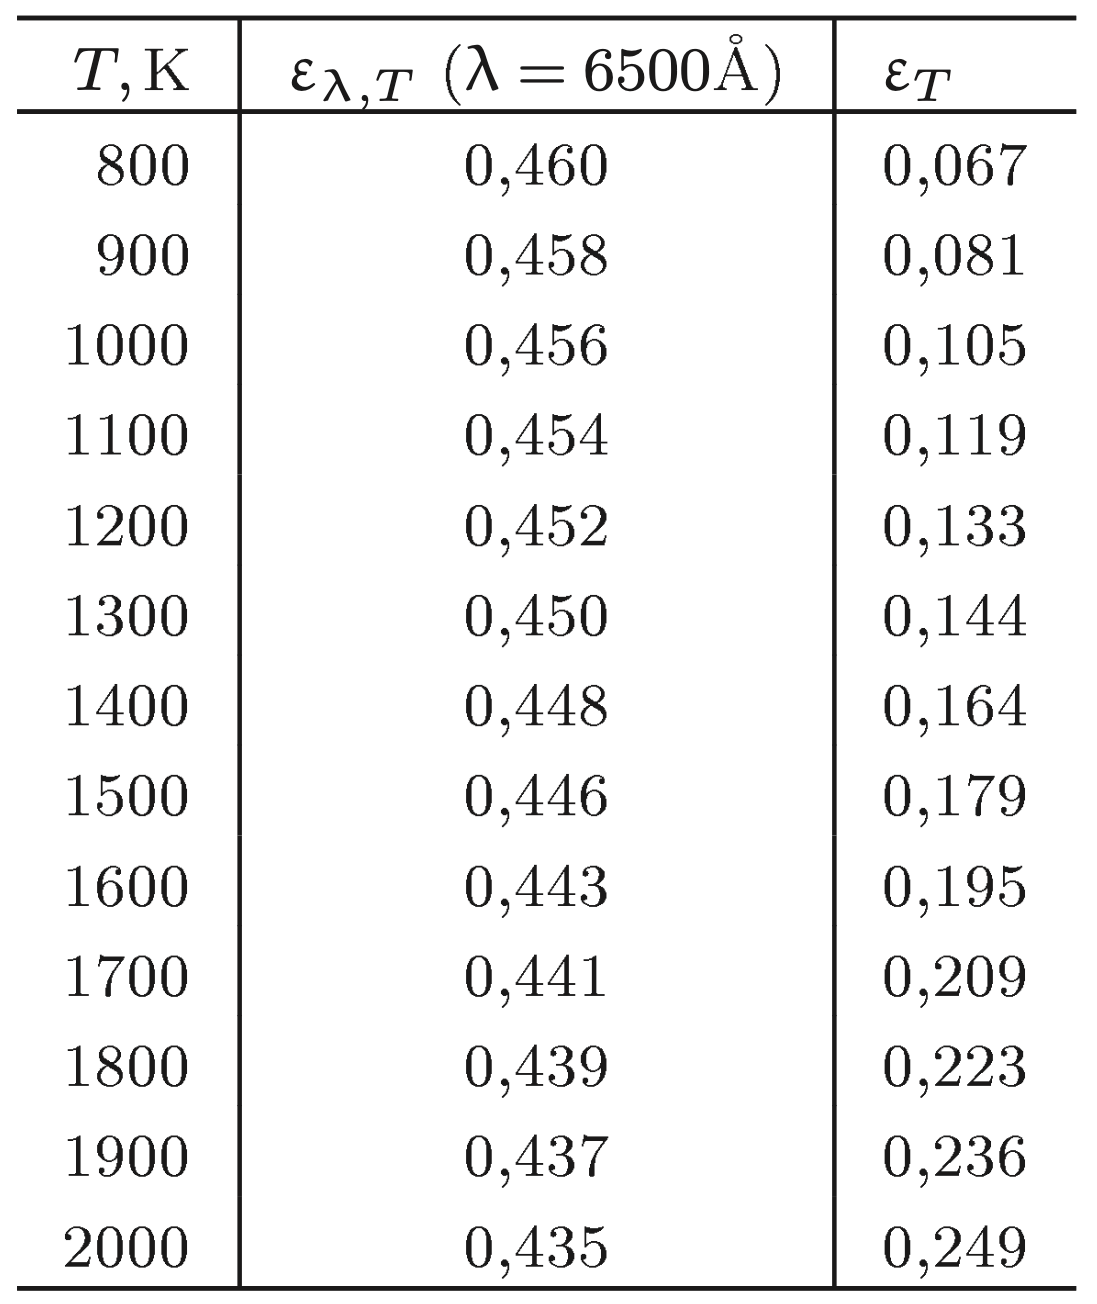
\includegraphics[width=\linewidth]{2}
    \captionsetup{justification =
    centering}
    \caption{График зависимости
    $T_\text{эксп}$ от $T_\text{теор}$}
\end{figure}
Коэффициент наклона прямой равен:
\[
k = 1,00 \pm 0,08
\]

Сопротивление контура $R_\text{конт}$
определяется как сумма сопротивления
магазина. Объединим данные из таблицы 2
и таблицы 3 и рассчитаем значения:
$1/R_\text{конт}^2$, $1/\Theta^2$ и их
погрешности. Сопротивление катушки $R_L$
взято при частоте $\nu = 5\ \text{кГц}$.
\begin{table}[H]
\begin{tabular}{|c|c|c|c|c|}
\hline
$R_\text{конт}, \ \text{Ом}$  & $1/\Theta^2$  &
$\Delta (1/\Theta^2)$ &
\begin{tabular}{c}
    $1/R^2_\text{конт}$, \\ $\text{Ом}^{-2} \cdot 10^6$  
\end{tabular}
& 
\begin{tabular}{c}
$\Delta
(1/R^2_\text{конт}),$\\
$\text{Ом}^{-2}
\cdot 10^6$  
\end{tabular}
\\ \hline
981  & 2,62 & 0,48 & 1,0392 & 0,0042 \\ \hline
1018 & 2,78 & 0,51 & 0,9650 & 0,0039 \\ \hline
1071 & 1,70 & 0,34 & 0,8718 & 0,0035 \\ \hline
1173 & 1,78 & 0,36 & 0,7268 & 0,0029 \\ \hline
1271 & 1,40 & 0,15 & 0,6190 & 0,0025 \\ \hline
1461 & 1,08 & 0,24 & 0,4685 & 0,0019 \\ \hline
1571 & 1,10 & 0,13 & 0,4052 & 0,0016 \\ \hline
1749 & 0,75 & 0,20 & 0,3269 & 0,0013 \\ \hline
1941 & 0,55 & 0,15 & 0,2654 & 0,0011 \\ \hline
1971 & 0,53 & 0,07 & 0,2574 & 0,0010 \\ \hline
2133 & 0,57 & 0,16 & 0,2198 & 0,0009 \\ \hline
2271 & 0,57 & 0,08 & 0,1939 & 0,0008 \\ \hline
2421 & 0,37 & 0,11 & 0,1706 & 0,0007 \\ \hline
2471 & 0,40 & 0,07 & 0,1638 & 0,0007 \\ \hline
2621 & 0,31 & 0,05 & 0,1456 & 0,0006 \\ \hline
2821 & 0,33 & 0,06 & 0,1257 & 0,0005 \\ \hline
2901 & 0,25 & 0,09 & 0,1188 & 0,0005 \\ \hline
\end{tabular}
\captionsetup{justification=centering}
\caption{Зависимость величины, обратной
к квадрату декремента $1/\Theta^2$ от
величины обратной к квадрату
сопротивления контура $1/R^2_\text{конт}$}
\end{table}

\begin{figure}[H]
    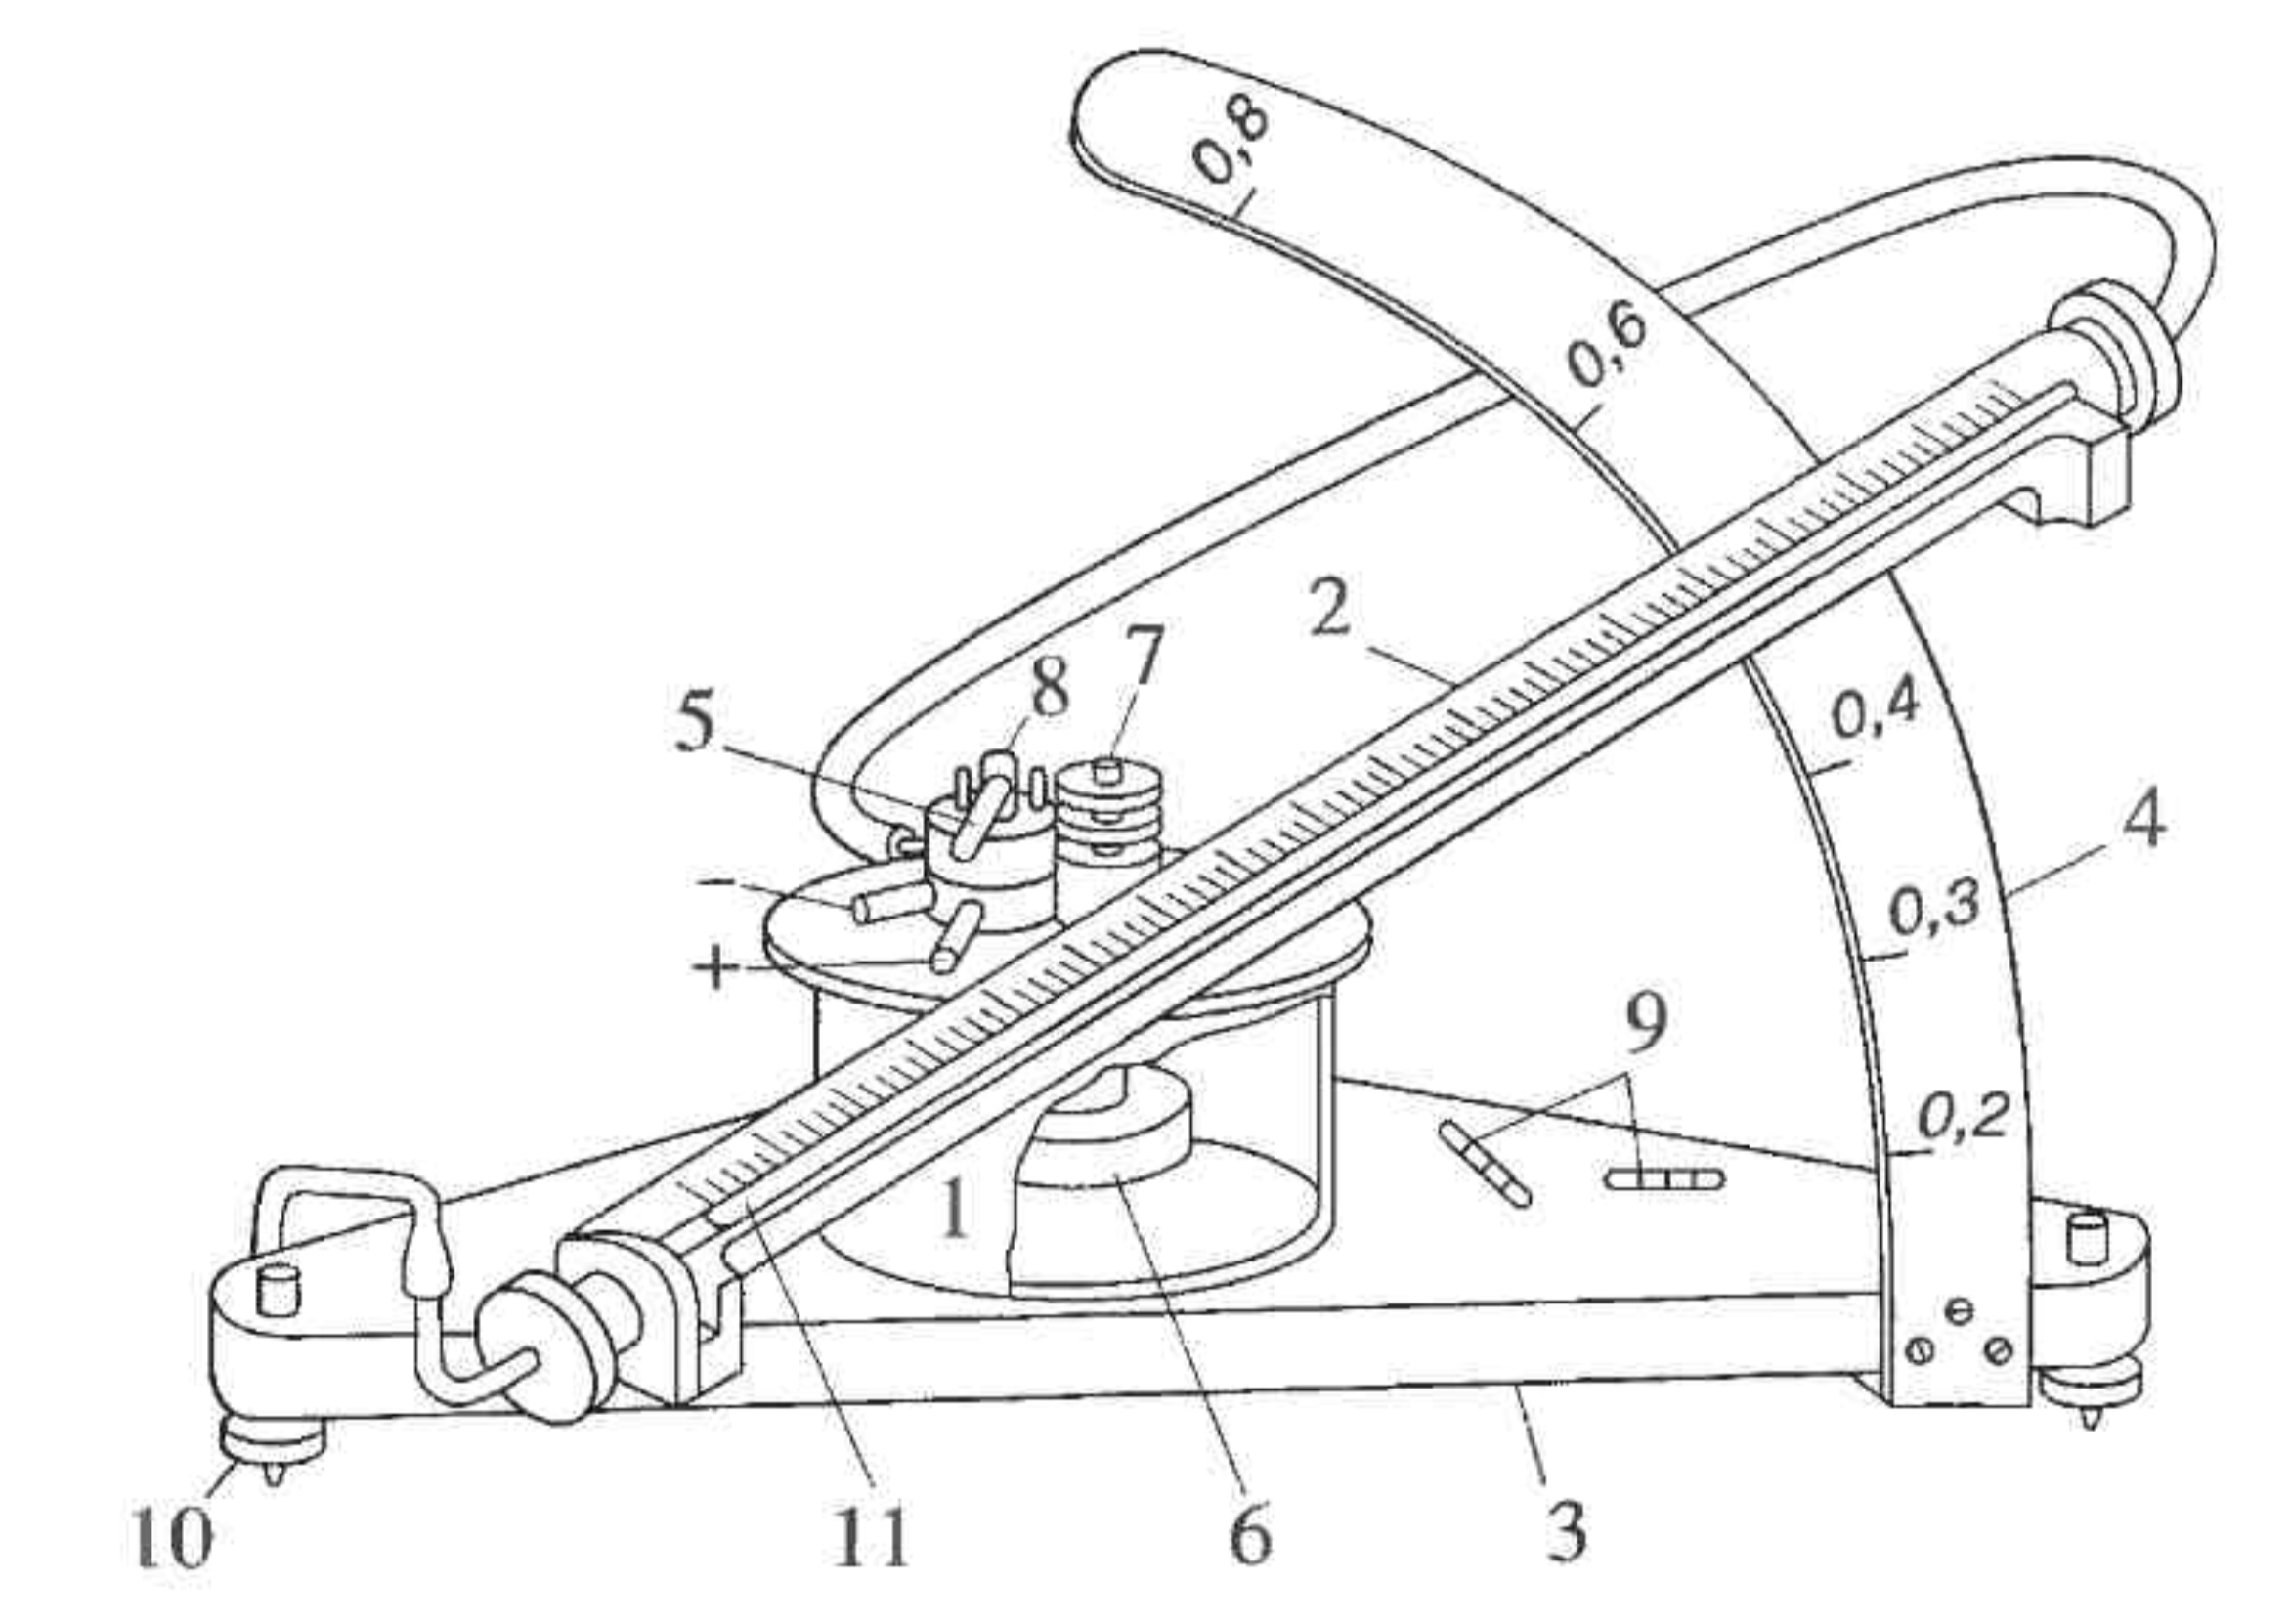
\includegraphics[width=\linewidth]{3}
    \captionsetup{justification=centering}
    \caption{График зависимости величины, обратной
к квадрату декремента $1/\Theta^2$ от
величины обратной к квадрату
сопротивления контура $1/R^2_\text{конт}$}
\end{figure}

По коэффициенту наклона рассчитаем
$R_\text{кр}$ по формуле $R_\text{кр} =
2\pi\sqrt{\Delta Y/\Delta X}$, где
$\Delta Y = \Delta (1/\Theta^2)$,
$\Delta X = \Delta (1/R_\text{конт}^2)$
\[
    R_\text{кр} = 10000 \pm 2000 \
    \text{Ом}
\]
Рассчитаем теоретическое значение
критического сопротивления
$R_\text{кр}^\text{т} = 2\sqrt{L/C}$. $C
= 5\ \text{нФ}$, $\nu = 5\ \text{кГц}$
 \[
R_\text{кр}^\text{т} = 10400 \pm 400 \
\text{Ом}
\]

Рассчитаем добротность контура $Q$ по
формуле $Q = \pi/\Theta$ для
максимального и минимального значений
$\Theta$ по картине затухающих
колебаний (данные из таблицы 2). Также
произведем расчеты добротности
$Q^\text{конт}$ по формуле $Q =
1/R\sqrt{L/C}$

\begin{equation*}
    \begin{aligned}
        Q_{min} = 1,6 \pm 0,3; \qquad& 
        Q_{min}^\text{конт} = 1,812 \pm
        0,007 \\
        Q_{max} = 5,1 \pm 0,5;  \qquad &
        Q_{max}^\text{конт} = 5,44 \pm
        0,02
    \end{aligned}
\end{equation*}

Выполним расчет добротности $Q$ по
значениям декремента затухания при
наблюдении колебаний на фазовой
плоскости (таблица 3)
\begin{equation*}
    \begin{aligned}
        Q_{min}^\text{сп} &= 1,76 \pm 0,15 \\
        Q_{max}^\text{сп} &= 5,3 \pm 0,4
    \end{aligned}
\end{equation*}


\section{Обсуждение результатов и выводы}

В работе была исследована
зависимость периода свободных
колебаний контура от ёмкости
(Таблица 1). По результатам 
был построен график зависимости
периода колебаний контура, найденного
экспериментально $T_\text{эксп}$, от теоретического
значения периода колебаний
$T_\text{теор}$ (Рис. 2). Из
графика коэффициент наклона прямой $k$:
\[
k = 1,00 \pm 0,08
\]
что свидетельствует о совпадении
экспериментального и теоретического
значений периода колебаний контура

Была исследована зависимость
логарифмического декремента
затухания $\Theta$ от сопротивления
контура $R$. (Рис 3)

Разными способами было определено
критическое сопротивление контура
$R_\text{кр}$, а также его
добротность $Q$.
\begin{table}[H]
\begin{tabular}{|c|c|c|c|}
\hline
\multirow{2}{*}{$L_\text{кат}, \
\text{мГн}$} &
\multicolumn{3}{c|}{$R_\text{кр}, \
\text{Ом}$}                          \\ \cline{2-4}
                   &
Теор.               &
Подбор            &
Граф.             \\ \hline
$137 \pm 3$          & $10400 \pm 400$   &
$9800 \pm 800$ & $10000 \pm 2000$ \\ \hline
\hline
\multirow{2}{*}{$R, \ \text{Ом}$} & \multicolumn{3}{c|}{Q}                          \\ \cline{2-4}
                   &
Теор.             &
$f(\Theta)$           & Спираль 
\\ \hline
2880               & $5,44 \pm 0,02$   &
$5,1 \pm 0,5$  & $5,3 \pm 0,4$    \\ \hline
960                & $1,812 \pm 0,007$ &
$1,6 \pm 0,3$  & $1,76 \pm 0,15$  \\ \hline
\end{tabular}
\end{table}
\end{document}
